\subsection{Addresses}

\begin{figure}[ht]
    \centering
    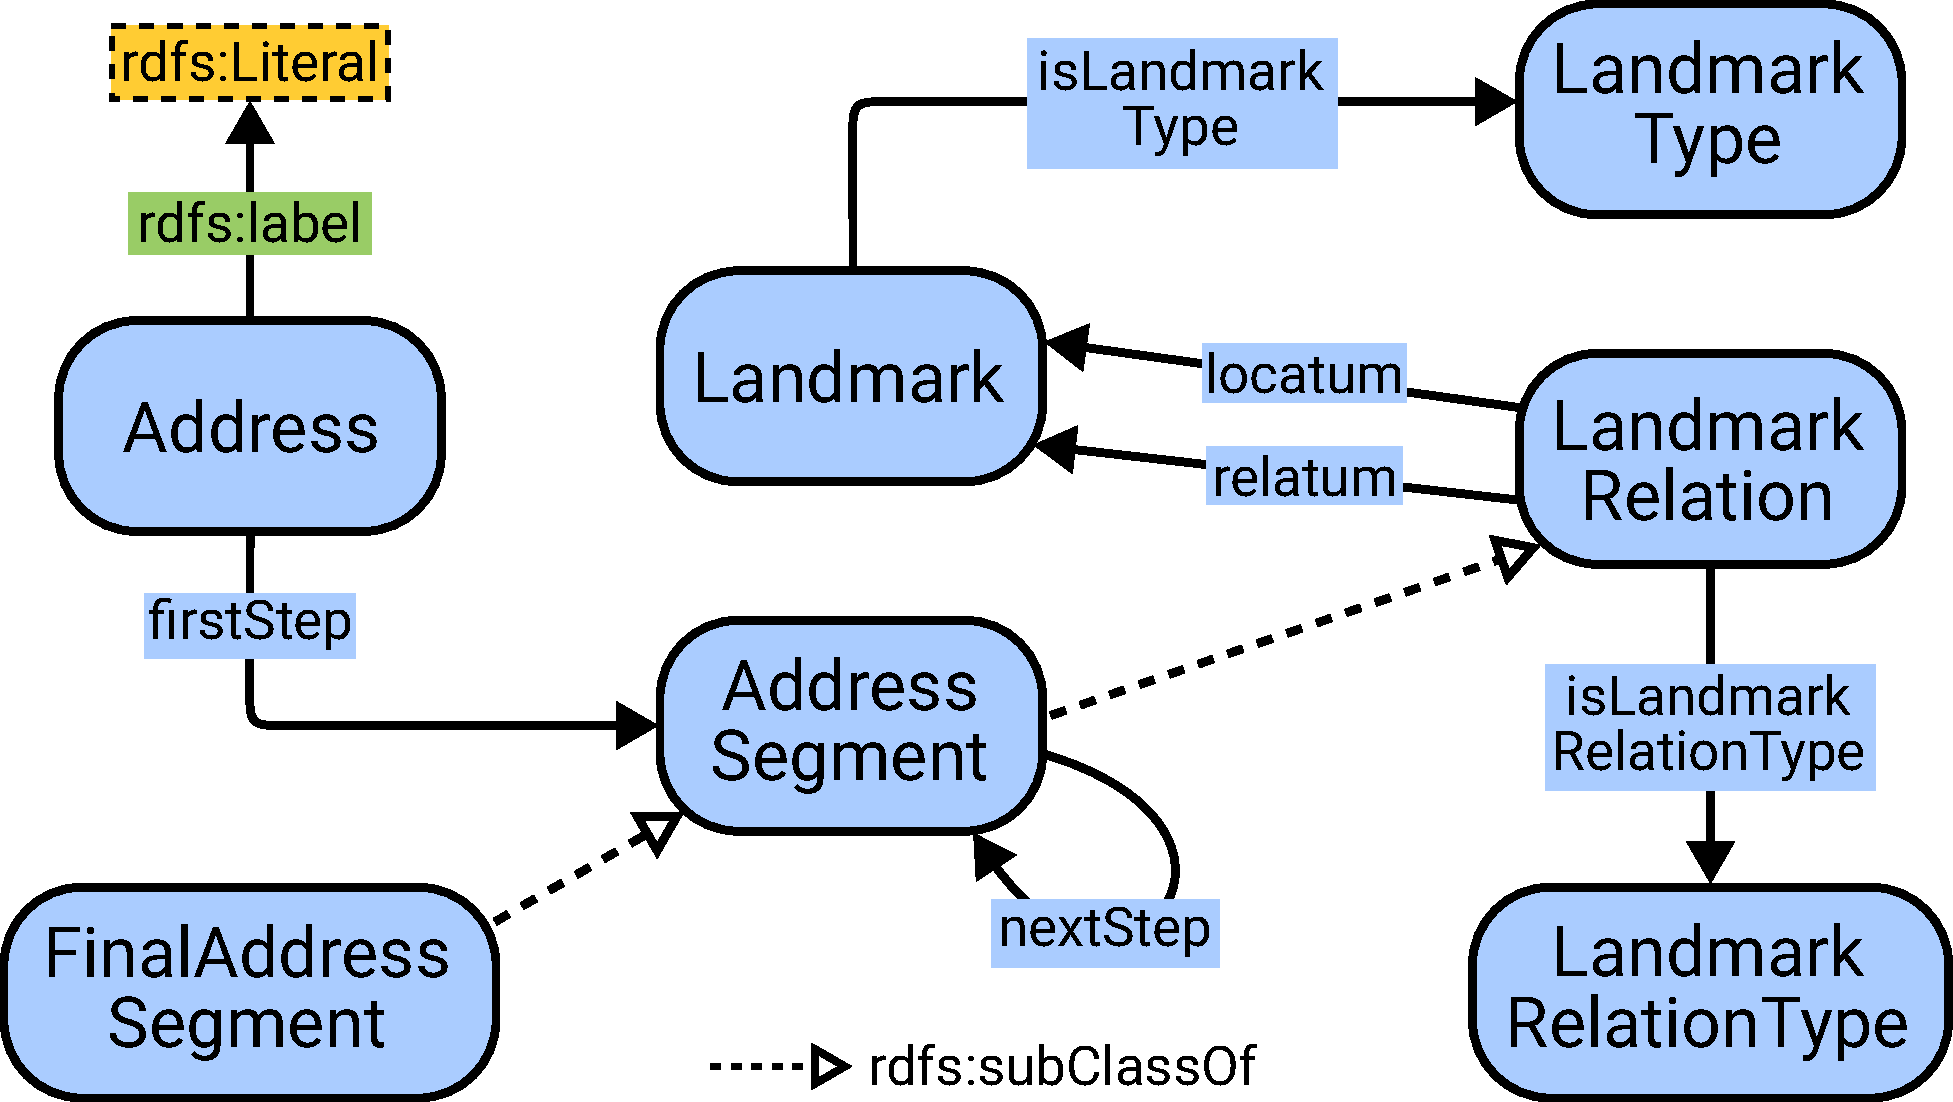
\includegraphics[width=0.8\textwidth]{images/address_ont.pdf}
    \caption{Simplified representation of the ontology.}
    \label{fig:address_ont}
\end{figure}

\begin{figure}[ht]
    \centering
    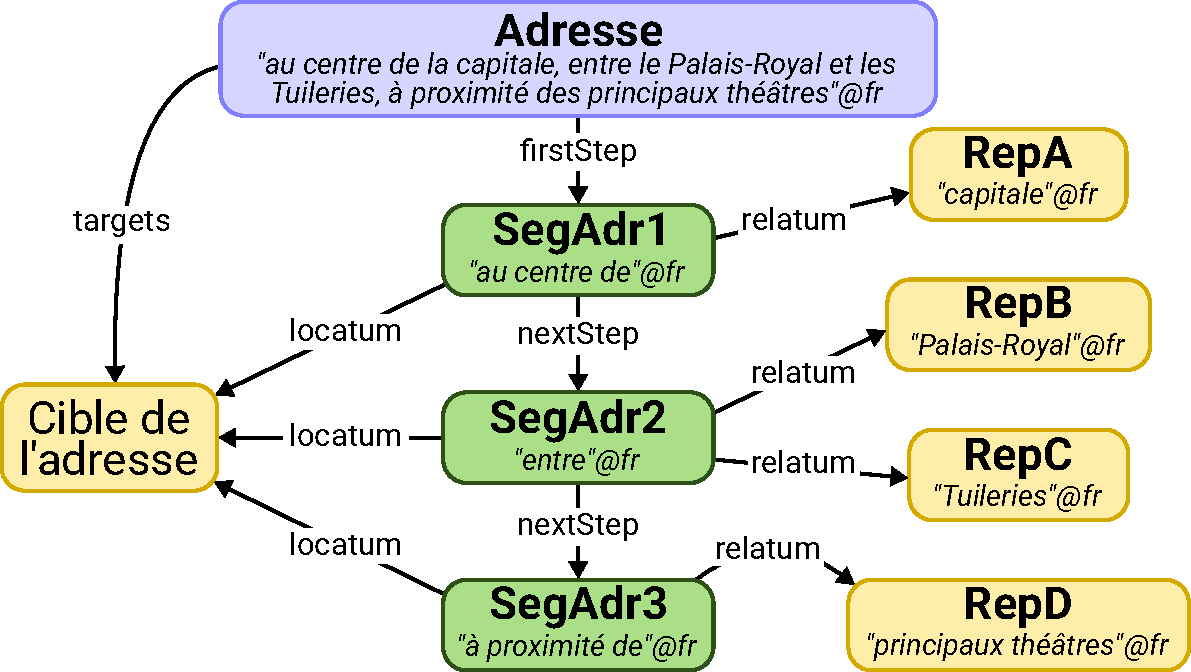
\includegraphics[width=0.9\textwidth]{images/exemple_modelisation_adresse.pdf}
    \caption{Example of address modelling.}
    \label{fig:exemple_modelisation_adresse}
\end{figure}

In this modelet\footnote{\texttt{https://github.com/charlybernard/phd-ontologie}}, an address is composed of references to spatial landmarks, connected by spatial relationships, which together point to a target location to which geographic coordinates can be associated.
Therefore, we selected the following competency questions:
(1) what are the addresses listed along a given street?
(2) what are the coordinates corresponding to the target of a given address?
(3) what are the addresses located within a given area?

The ontology, presented in Figure~\ref{fig:address_ont}, contains three concepts:
\begin{itemize}
    \item the address (\texttt{Address}), corresponding to the statement describing a location;
    \item the address segment (\texttt{AddressSegment}), a subclass of~\texttt{LandmarkRelation}, describing a relation between landmarks involved in an address. The nature of this relation is defined by~\texttt{LandmarkRelationType};
    \item the landmark (\texttt{Landmark}), describing a geographic entity. \texttt{LandmarkType} defines its nature (e.g., administrative unit, street, house number, building, etc.).
\end{itemize}

The location designated by an address is represented as a~\texttt{Landmark}, while the sequence of geographic references composing the address is represented through resources of type~\texttt{AddressSegment} which is a subclass of~\texttt{LandmarkRelation}, each segment represents a typed relation between two landmarks.

A resource of type~\texttt{Address} is linked through the property~\texttt{firstStep} to the first resource of type~\texttt{AddressSegment}. Each segment is then linked through the property~\texttt{nextStep} to the following segment, and so on. The type of relation represented by each segment is specified using~\texttt{LandmarkRelationType}. To represent the end of this sequence, the last resource is typed as~\texttt{FinalAddressSegment}, a subclass of~\texttt{AddressSegment}.

A resource of type~\texttt{AddressSegment} describes a step in the path linking a landmark, called the \textit{locatum}, to one or more landmarks called \textit{relatum}~\cite{tenbrink_model_2011}.
Generally, the locatum corresponds to the target of the address, as each step of the path aims to provide additional information about its location.
The example presented in Figure~\ref{fig:exemple_modelisation_adresse} illustrates this principle.
The address points to an unknown landmark and has a label that can be divided into three parts:
"\textit{in the centre of the capital}",
"\textit{between the Palais-Royal and the Tuileries}",
and
"\textit{near the main theatres}".
There are three address segments and four references to geographic landmarks.

\subsection{Temporal evolution}
\label{sect:prop_evolution_temporelle}

\begin{figure}[ht]
\begin{center}
 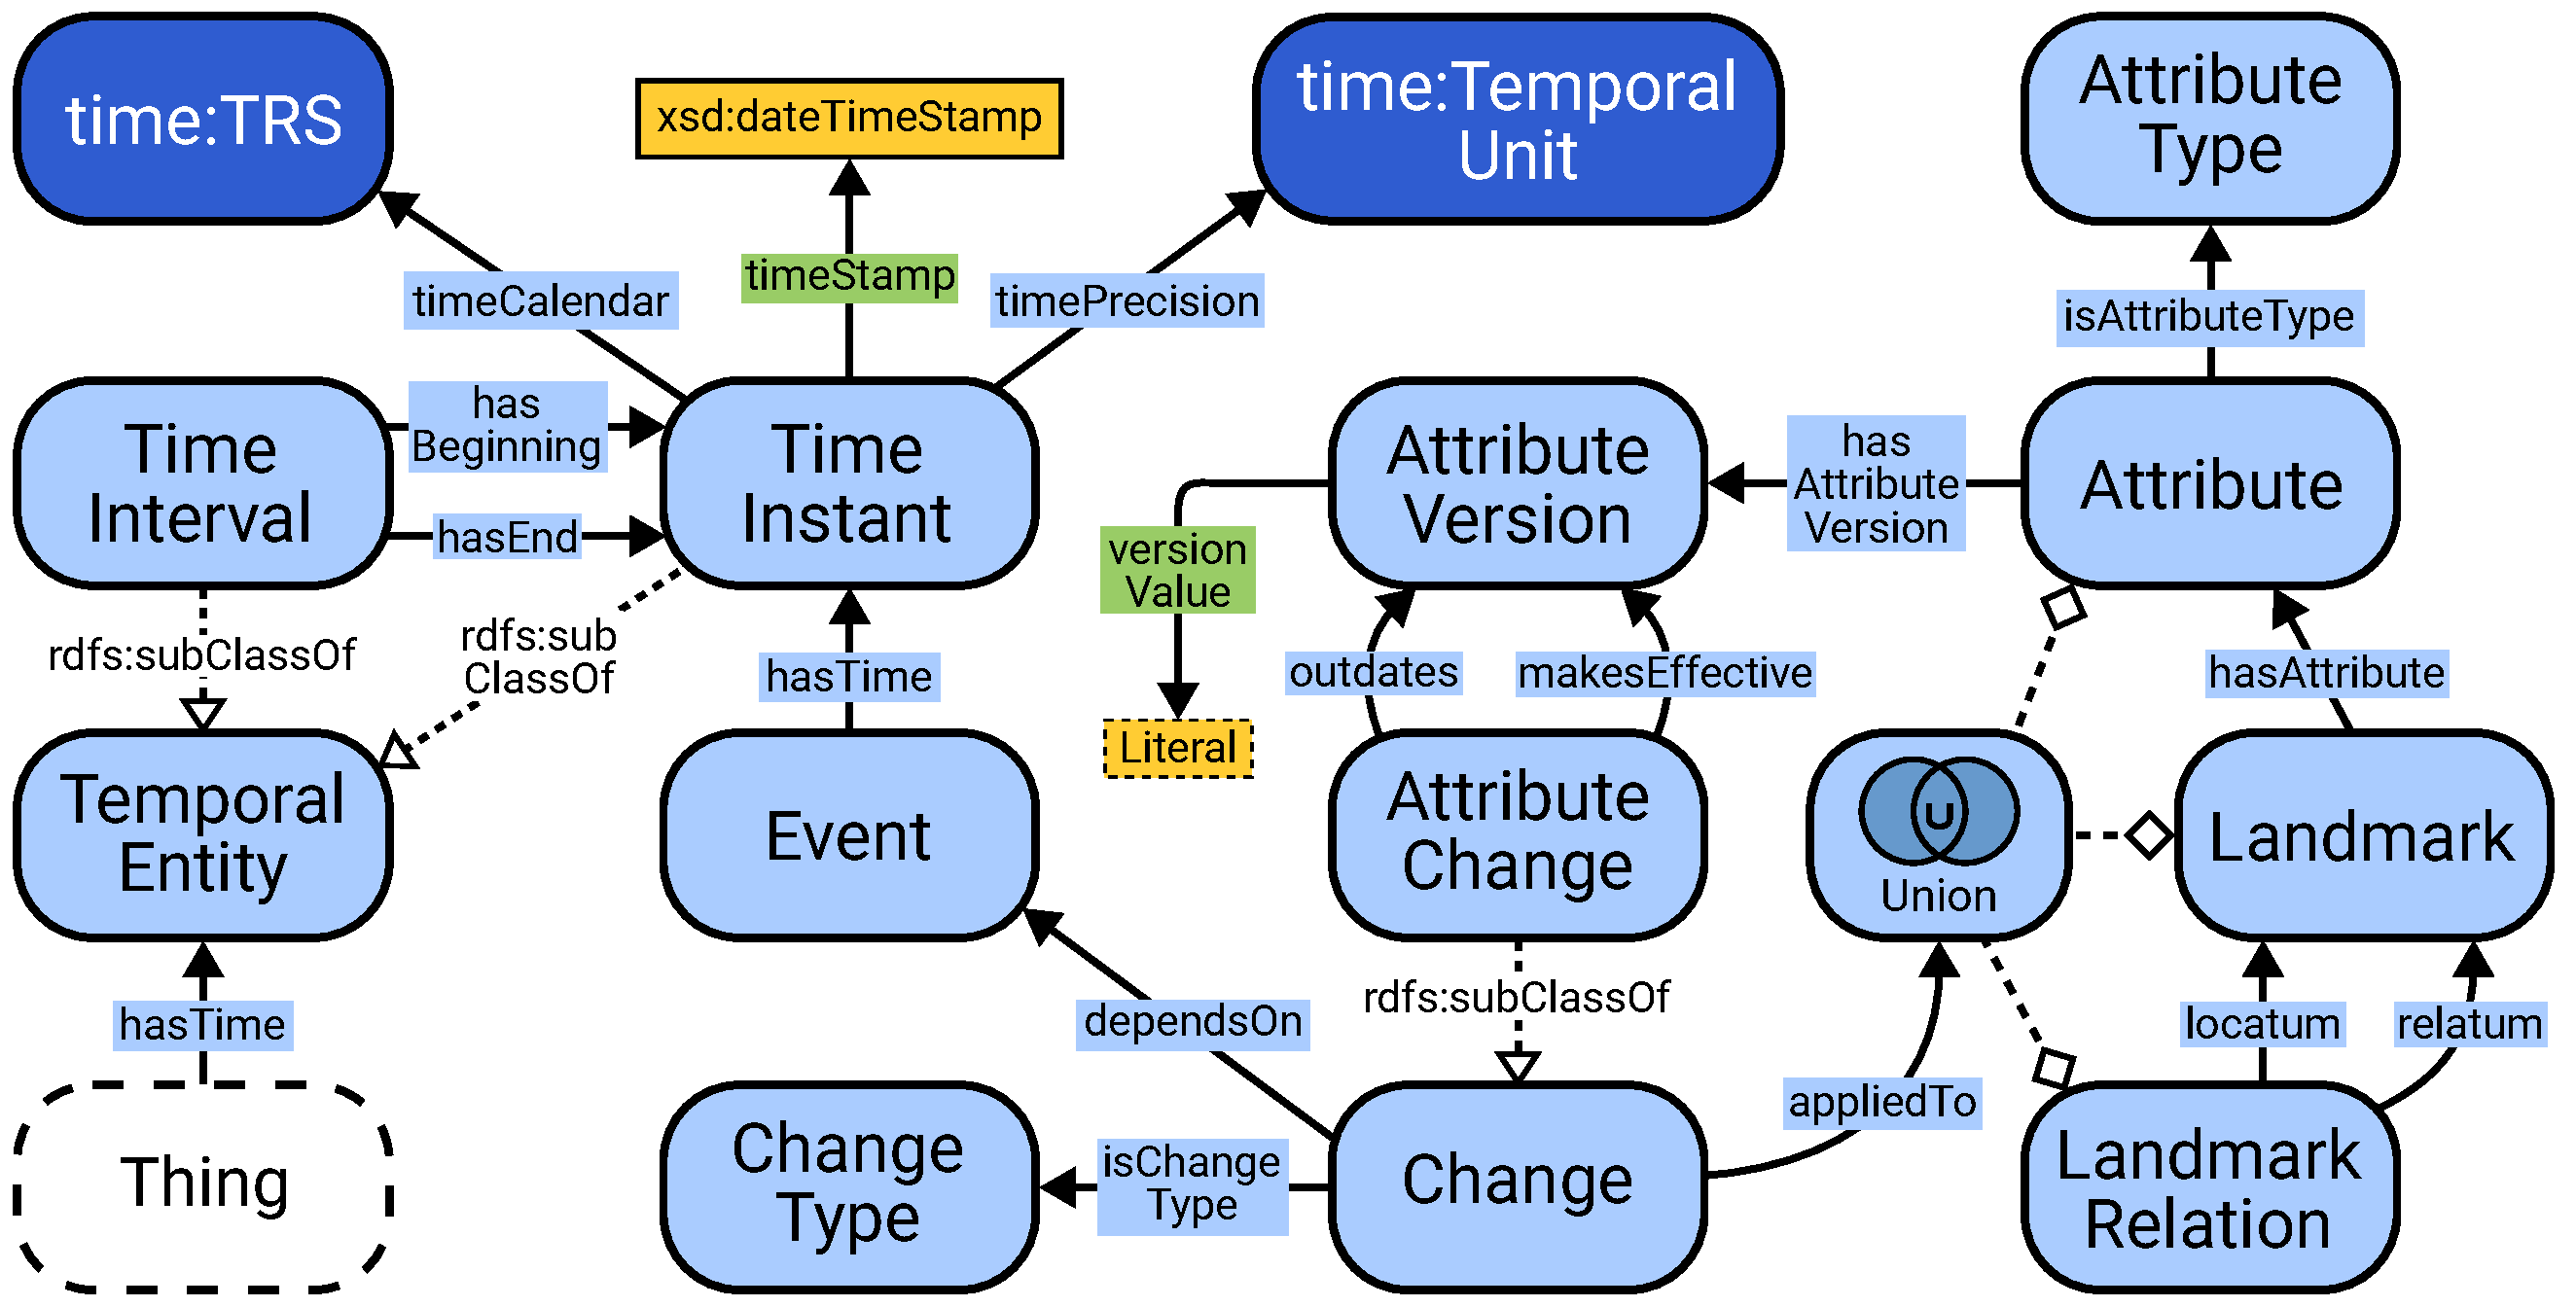
\includegraphics[width=\textwidth]{images/events_ont.pdf}
 \caption[]{Representation of the ontology for the temporal evolution of geographic landmarks\footnotemark.} 
\label{fig:events_ont}
\end{center}
\end{figure}

\footnotetext{The element linked to the class \texttt{Change} through the predicate \texttt{appliedTo} describes the union of \texttt{Attribute} and \texttt{Landmark}.}

For this modelet, we identified the following competency questions:
(1) which streets exist at a given time?
(2) over which temporal interval(s) is a given address name valid?
(3) what is the history of a landmark? In other words, which events are associated with it?
(4) which states and events are missing from the history of an address?

Two main requirements emerge from these competency questions:
the ability to retrieve the state of geographic landmarks at any given time, and the representation of events that have affected geographic landmarks and their properties.

For the second aspect, we draw inspiration from the work of~\cite{bernard_ontologies_2018} by decomposing events into elementary changes that explicitly describe the transition between two versions.
In addition to applying changes to landmarks, we chose to associate changes with landmark attributes.
This makes it possible to determine the evolution of a specific attribute.
For this purpose, a property associated with a landmark is represented through a resource of type~\texttt{Attribute}, to which versions are attached.
Whenever a change affects a landmark or one of its attributes, it is represented by a resource of type~\texttt{Change}, which specifies the resource affected by the change.

\cite{bernard_ontologies_2018} studies the evolution of entities through \textit{snapshots}, meaning that changes describe the evolution between two successive versions of an entity, even when no difference exists between them.
This approach is discrete, whereas our objective is to assign each entity its own validity time in order to describe the state of the territory at any given moment, which is enabled by our modelling.

Figure~\ref{fig:events_ont} presents the four main concepts of the ontology:

\begin{enumerate}
    \item the change (\texttt{Change}), which describes an elementary operation of an event. If it applies to a geographic landmark, the change is a \texttt{LandmarkChange}; if it applies to an attribute (such as the name of a street), it is an \texttt{AttributeChange}. \texttt{ChangeType} defines its type (e.g., appearance or disappearance of a landmark);
    \item the attribute (\texttt{Attribute}), whose type is defined by \texttt{AttributeType};
    \item the attribute version (\texttt{AttributeVersion}).
\end{enumerate}

\begin{figure}[ht]
\begin{center}
 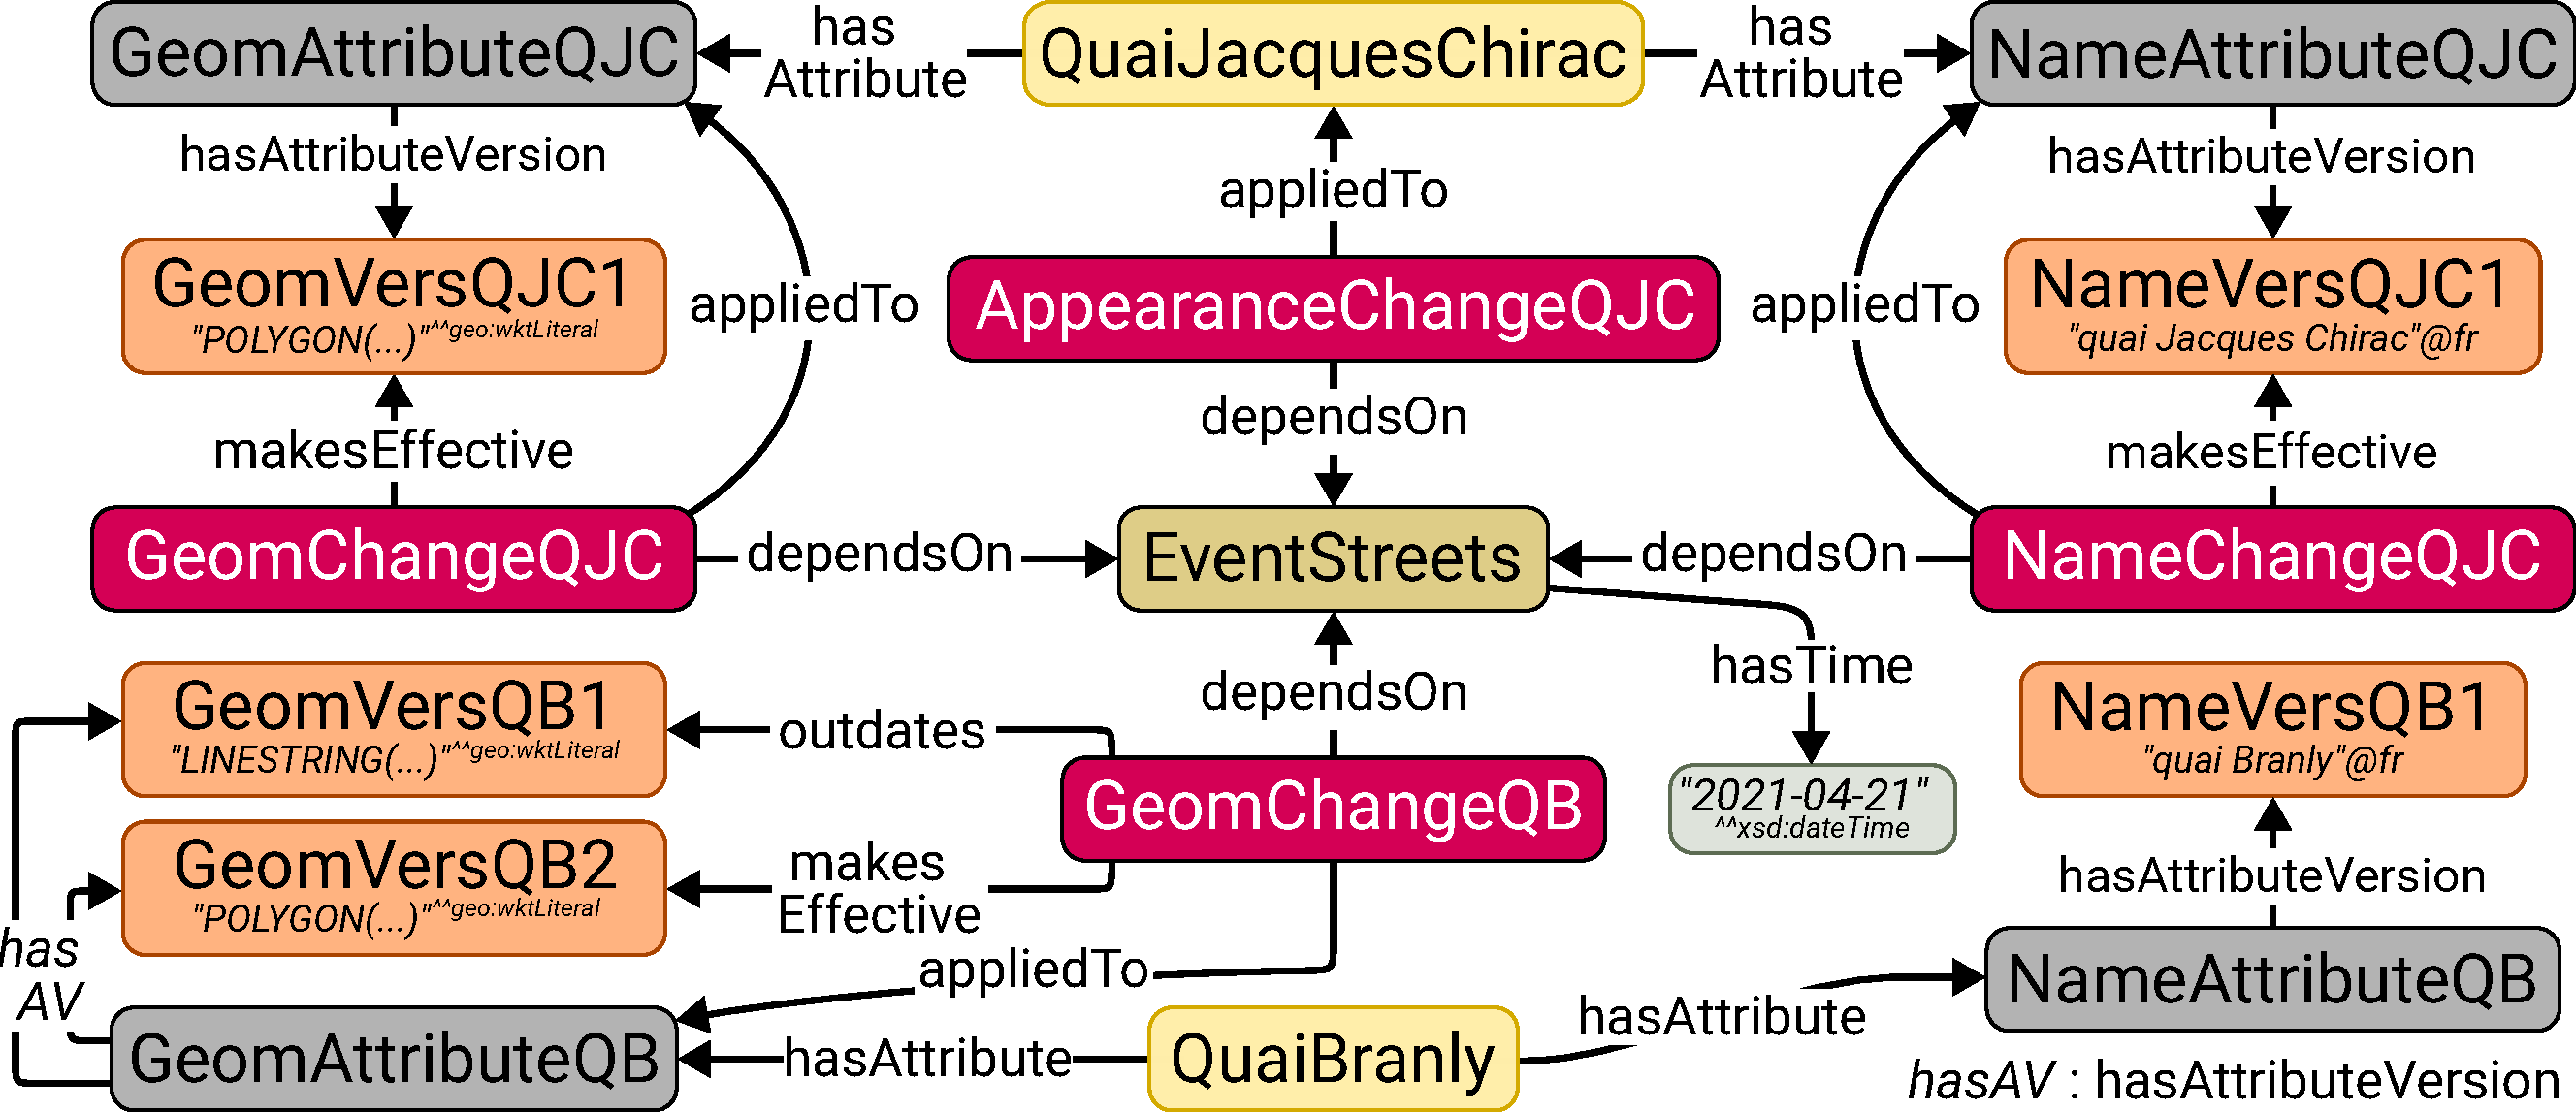
\includegraphics[width=\textwidth]{images/exemple_modelisation_temporelle.pdf}
 \caption{Example of modelling the joint evolution of two streets: creation of \textit{quai Jacques Chirac} through the subdivision of \textit{quai Branly}.}
 \label{fig:exemple_modelisation_temporelle}
\end{center}
\end{figure}

With this modelling, modifications involving one or several geographic entities can be decomposed into elementary changes.
Consider the event "creation of quai Jacques Chirac from a portion of quai Branly on April 21, 2021".
As represented in Figure~\ref{fig:exemple_modelisation_temporelle}, it can be divided into several changes:

\begin{itemize}
    \item appearance of the landmark \texttt{QuaiJacquesChirac};
    \item creation of a new version of \texttt{NameAttributeQJC}, a name attribute, for which no previous version exists;
    \item creation of a new version of \texttt{GeomAttributeQJC}, a geometry attribute, also without a previous version;
    \item creation of a new version of \texttt{GeomAttributeQB}, the geometry attribute of quai Branly, whose previous version corresponded to the spatial extent of the quay from Place de la Résistance to Pont d'Iéna.
\end{itemize}